\section{Hasil Simulasi dan Optimasi}
\label{sec:hasil-simulasi-optimasi}

Proses optimasi dilakukan secara simultan dengan simulasi variasi durasi gangguan cuaca dan variasi konsumsi harian BBM. Standar simulasi yang dilakukan dalam pengerjaan tugas akhir ini adalah 1000 iterasi untuk satu kali simulasinya. Skenario yang dilakukan ada dua jenis, yaitu usulan sistem pemasokan baru tanpa pengembangan tangki dan dengan pengembangan tangki penyimpanan di pelabuhannya. Hasil simulasi dapat dilihat pada tabel \ref{tabel:ringkasan-hasil}, sedangkan untuk bentuk distribusi masing-masing variabel dapat dilihat pada pembahasan selanjutnya.

\begin{table}[!ht]
    \centering
    \caption{Ringkasan Hasil Simulasi Skenario}
    \label{tabel:ringkasan-hasil}
    \begin{tabular}{|cccccc|}
    \hline
    \multicolumn{6}{|c|}{TANPA TANGKI}                                                                                                                                                           \\ \hline
    \multicolumn{1}{|c|}{Variabel}                & \multicolumn{1}{c|}{Satuan}      & \multicolumn{1}{c|}{Min.}     & \multicolumn{1}{c|}{Mean}     & \multicolumn{1}{c|}{Max.}     & STD. DEV. \\ \hline
    \multicolumn{1}{|c|}{Biaya Tahunan}           & \multicolumn{1}{c|}{Juta Rupiah} & \multicolumn{1}{c|}{8.480,25} & \multicolumn{1}{c|}{8.574,22} & \multicolumn{1}{c|}{8.671,27} & 35,12     \\ \hline
    \multicolumn{1}{|c|}{Biaya Publik}            & \multicolumn{1}{c|}{Juta Rupiah} & \multicolumn{1}{c|}{43,47}    & \multicolumn{1}{c|}{882,86}   & \multicolumn{1}{c|}{2.988,31} & 162,39    \\ \hline
    \multicolumn{1}{|c|}{Frekuensi}               & \multicolumn{1}{c|}{Trip}        & \multicolumn{1}{c|}{15}       & \multicolumn{1}{c|}{15,80}    & \multicolumn{1}{c|}{17}       & 0,49      \\ \hline
    \multicolumn{1}{|c|}{Port Calls}              & \multicolumn{1}{c|}{Kunjungan}   & \multicolumn{1}{c|}{66}       & \multicolumn{1}{c|}{70,14}    & \multicolumn{1}{c|}{74}       & 1,58      \\ \hline
    \multicolumn{1}{|c|}{Kekurangan Bensin}       & \multicolumn{1}{c|}{kiloliter}   & \multicolumn{1}{c|}{0,20}     & \multicolumn{1}{c|}{16,06}    & \multicolumn{1}{c|}{54,32}    & 8,82      \\ \hline
    \multicolumn{1}{|c|}{Kekurangan Minyak Tanah} & \multicolumn{1}{c|}{kiloliter}   & \multicolumn{1}{c|}{0}        & \multicolumn{1}{c|}{27,26}    & \multicolumn{1}{c|}{104,86}   & 24,13     \\ \hline
    \multicolumn{1}{|c|}{Kekurangan Solar}        & \multicolumn{1}{c|}{kiloliter}   & \multicolumn{1}{c|}{0}        & \multicolumn{1}{c|}{1,02}     & \multicolumn{1}{c|}{10,63}    & 1,44      \\ \hline
    \multicolumn{6}{|c|}{{\color[HTML]{000000} DENGAN TANGKI}}                                                                                                                                   \\ \hline
    \multicolumn{1}{|c|}{Biaya Tahunan}           & \multicolumn{1}{c|}{Juta Rupiah} & \multicolumn{1}{c|}{8.051,64} & \multicolumn{1}{c|}{8.140,05} & \multicolumn{1}{c|}{8.251,89} & 32,25     \\ \hline
    \multicolumn{1}{|c|}{Biaya Publik}            & \multicolumn{1}{c|}{Juta Rupiah} & \multicolumn{1}{c|}{0}        & \multicolumn{1}{c|}{410,04}   & \multicolumn{1}{c|}{2.417,93} & 115,40    \\ \hline
    \multicolumn{1}{|c|}{Frekuensi}               & \multicolumn{1}{c|}{Trip}        & \multicolumn{1}{c|}{7}        & \multicolumn{1}{c|}{7,75}     & \multicolumn{1}{c|}{8}        & 0,43      \\ \hline
    \multicolumn{1}{|c|}{Port Calls}              & \multicolumn{1}{c|}{Kunjungan}   & \multicolumn{1}{c|}{27}       & \multicolumn{1}{c|}{31,60}    & \multicolumn{1}{c|}{34}       & 1,11      \\ \hline
    \multicolumn{1}{|c|}{Kekurangan Bensin}       & \multicolumn{1}{c|}{kiloliter}   & \multicolumn{1}{c|}{0}        & \multicolumn{1}{c|}{7,63}     & \multicolumn{1}{c|}{44,66}    & 6,68      \\ \hline
    \multicolumn{1}{|c|}{Kekurangan Minyak Tanah} & \multicolumn{1}{c|}{kiloliter}   & \multicolumn{1}{c|}{0}        & \multicolumn{1}{c|}{9,99}     & \multicolumn{1}{c|}{90,21}    & 16,22     \\ \hline
    \multicolumn{1}{|c|}{Kekurangan Solar}        & \multicolumn{1}{c|}{kiloliter}   & \multicolumn{1}{c|}{0}        & \multicolumn{1}{c|}{1,02}     & \multicolumn{1}{c|}{10,63}    & 1,44      \\ \hline
    \end{tabular}
    \end{table}


\subsection{Ukuran Utama Kapal Terpilih}
\label{subsec:ukuran-utama}

Hasil dari optimasi yang dilakukan dapat dilihat pada tabel \ref{tabel-hasil-maindim}. Ukuran utama ini yang akan digunakan untuk proses desain. Meskipun nanti ketika dilihat hasil analisis \emph{load factor} kapasitas kapal masih terlalu besar, akan tetapi karena konsideran utama penelitian ini adalah moda transportasi laut yang dapat memasok BBM dengan andal akhirnya \emph{constraint} yang diberikan bobot lebih tinggi saat pemilihan ukuran utama kapal adalah kemampuan mengghadapi gelombang. Disamping \emph{trade off} dari sisi ukuran tangki kapal, permintaan BBM yang sangat sedikit di Kabupaten Maluku Barat Daya juga menimbulkan hari operasional \emph{(seatime + porttime)} yang hanya sekitar 40 hari untuk sistem baru dengan tangki dan 80 hari untuk tanpa tangki. Kedua pengorbanan tersebut bisa dikompromikan dengan pengangkutan BBM bersamaan dengan komoditas lain atau dengan jenis moda kapal selain tanker dan SPOB sebagaimana yang sudah diteliti oleh senior penulis pada bab \ref{sec:penelitian-terkait}.

\begin{table}[!ht]
    \centering
    \caption{Tabel Ukuran Utama Hasil Optimasi}
    \begin{tabular}{|l|l|}
    \hline
        \textbf{LPP [m]} & 53,42 \\ \hline
        \textbf{Beam  [m]} & 8,52 \\ \hline
        \textbf{Depth  [m]} & 4,11 \\ \hline
        \textbf{Draught [m]} & 3,04 \\ \hline
        \textbf{Speed [Knot]} & 6,75 \\ \hline
        \textbf{Tangki  Bensin [$m^3$]} & 253,72 \\ \hline
        \textbf{Tangki Solar [$m^3$]} & 202,7 \\ \hline
        \textbf{Tangki Minyak Tanah [$m^3$]} & 396,74 \\ \hline
    \end{tabular}
    \label{tabel-hasil-maindim}
\end{table}

\subsection{Distribusi Ekspektasi Biaya Tahunan}
\label{subsec:annual-cost-dist}

Perubahan nilai tiap iterasi dari variabel konsumsi harian akan berdampak pada volume muatan yang harus dibawa, persediaan BBM di setiap titik dan berujung pada biaya penalti yang muncul akibat koreksi. Jumlah permintaan yang meningkat juga akan mempengaruhi biaya yang muncul akibat frekuensi perjalanan kapal bertambah.

\begin{figure}[!ht]
    \centering
    \begin{subfigure}{0.4\textwidth}
        \centering
        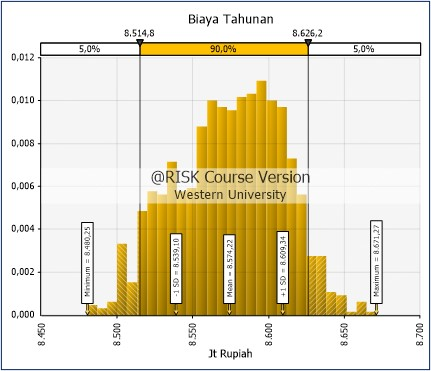
\includegraphics[width=\textwidth]{grafik/biaya-tahunan-baru.jpg}
        \caption{Tanpa Tangki}
    \end{subfigure}
    \hspace{0.04\textwidth}  % This adds horizontal spacing between images
    \begin{subfigure}{0.4\textwidth}
        \centering
        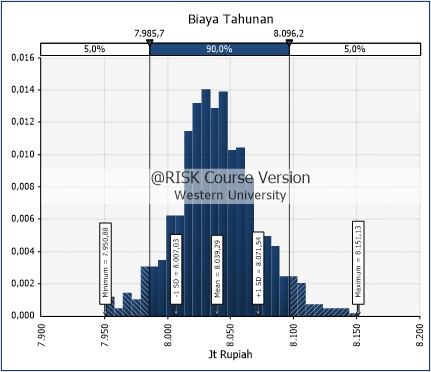
\includegraphics[width=\textwidth]{grafik/biaya-tahunan-baru-tangki.jpg}
        \caption{Dengan Tangki}    
    \end{subfigure}
    \caption{Hasil Simulasi Biaya}
    \label{fig:annual-cost-dist}
\end{figure}

Sistem pemasokan secara \emph{multiport} menyebabkan jarak yang ditempuh dalam setiap perjalanan berbeda sesuai dengan konsumsi BBM pada masing-masing titik. Investasi tangki menunjukkan biaya tahunan yang lebih murah dibandingkan dengan sistem tanpa tambahan tangki penyimpanan BBM di setiap titik. Penambahan tangki mampu memotong biaya perjalanan hingga setengah karena sinkronisasi waktu pemasokan di masing-masing titik. Persamaan waktu pemasokan tersebut membuat titik dengan permintaan yang tinggi seperti Tiakur harus sering dipasok.

\subsection{Analisis Kemungkinan Jumlah Perjalanan Tahunan}
\label{subsec:annual-freq-dist}

Frekuensi perjalanan setiap tahun dipengaruhi oleh angka konsumsi BBM harian dari setiap jenisnya. Model yang dibuat menentukan angka frekuensi berdasarkan ketika salah satu setiap jenis BBM habis dikonsumsi di salah satu titik maka harus diadakan pemasokan. Frekuensi tahunan akan mempengaruhi biaya tahunan dari sisi tambahan biaya perjalan yang muncul ketika kapal mengadakan pemasokan.

\begin{figure}[!ht]
    \centering
    \begin{subfigure}{0.4\textwidth}
        \centering
        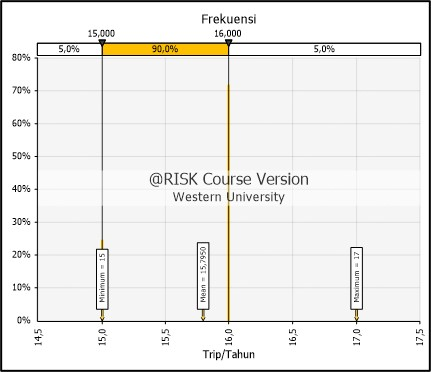
\includegraphics[width=\textwidth]{grafik/frekuensi-baru.jpg}
        \caption{Tanpa Tangki}
    \end{subfigure}
    \hspace{0.04\textwidth}  % This adds horizontal spacing between images
    \begin{subfigure}{0.4\textwidth}
        \centering
        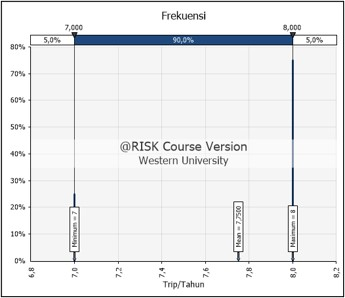
\includegraphics[width=\textwidth]{grafik/frekuensi-baru-tangki.jpg}
        \caption{Dengan Tangki}    
    \end{subfigure}
    \caption{Hasil Simulasi Frekuensi}
    \label{fig:annual-freq-dist}
\end{figure}

Gambar \ref{fig:annual-freq-dist} memperlihatkan bahwa kemungkinan frekuensi perjalanan dalam satu tahun relatif stabil di angka 7 dan 8 pada sistem baru dengan tambahan tangki. Selisih dua kali lipat dengan sistem tanpa tambahan investasi tangki. Unsur ini adalah titik utama penghematan antara sistem tanpa tangki dengan sistem dengan penambahan tangki.


\subsection{Analisis Kemungkinan Kelangkaan BBM}
\label{subsec:stock-out-over-capacity}

Proses yang sama seperti saat pengujian hipotesis dilakukan kembali dan diintegrasikan kedalam model untuk mendapatkan ukuran utama kapal yang optimal. Hasil simulasi menunjukkan bahwa jenis BBM solar cenderung tidak terjadi kelangkaan. Hal ini disebabkan konsumsi solar sangat kecil dibandingkan dengan minyak tanah dan bensin. Disisi lain hal ini menyebabkan \emph{load factor} solar cenderung kecil.

\begin{figure}[!ht]
    \centering
    \begin{subfigure}{0.95\textwidth}
        \centering
        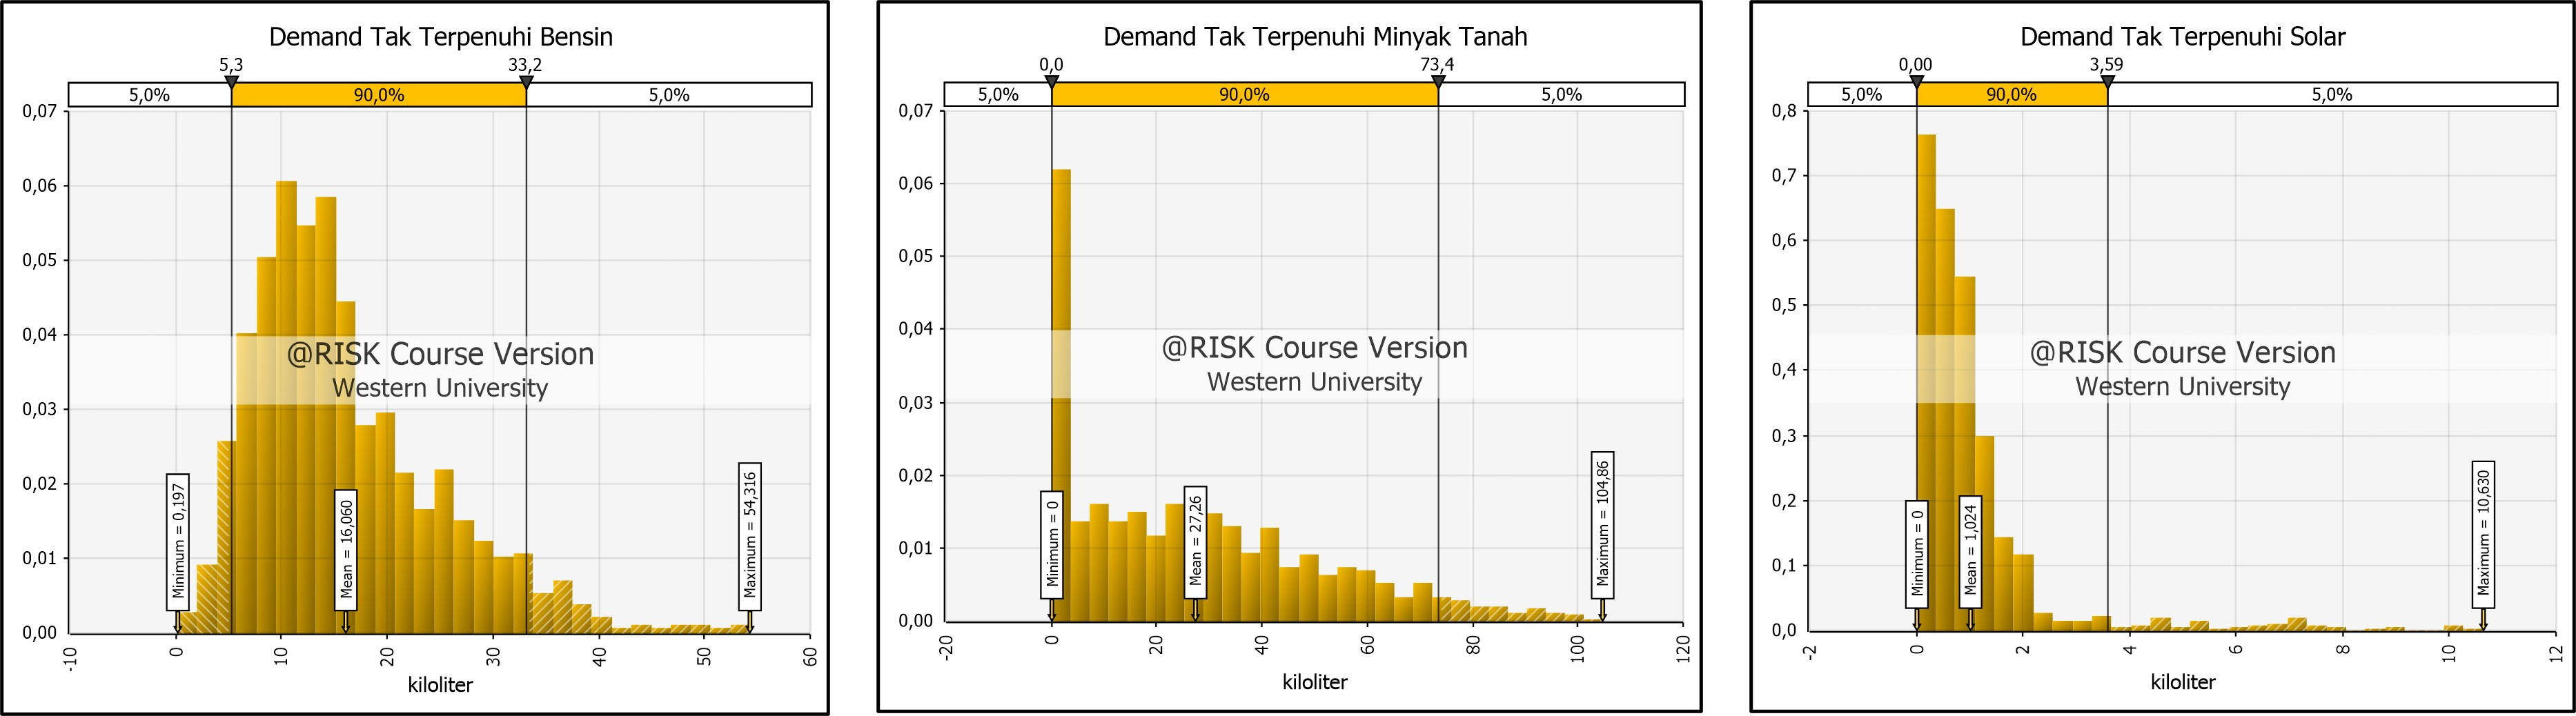
\includegraphics[width=\textwidth]{grafik/minus-bbm-baru.jpg}
        \caption{Tanpa Tangki}
    \end{subfigure}
    
    \vspace{0.3cm}  % Vertical space between images
    
    \begin{subfigure}{0.95\textwidth}
        \centering
        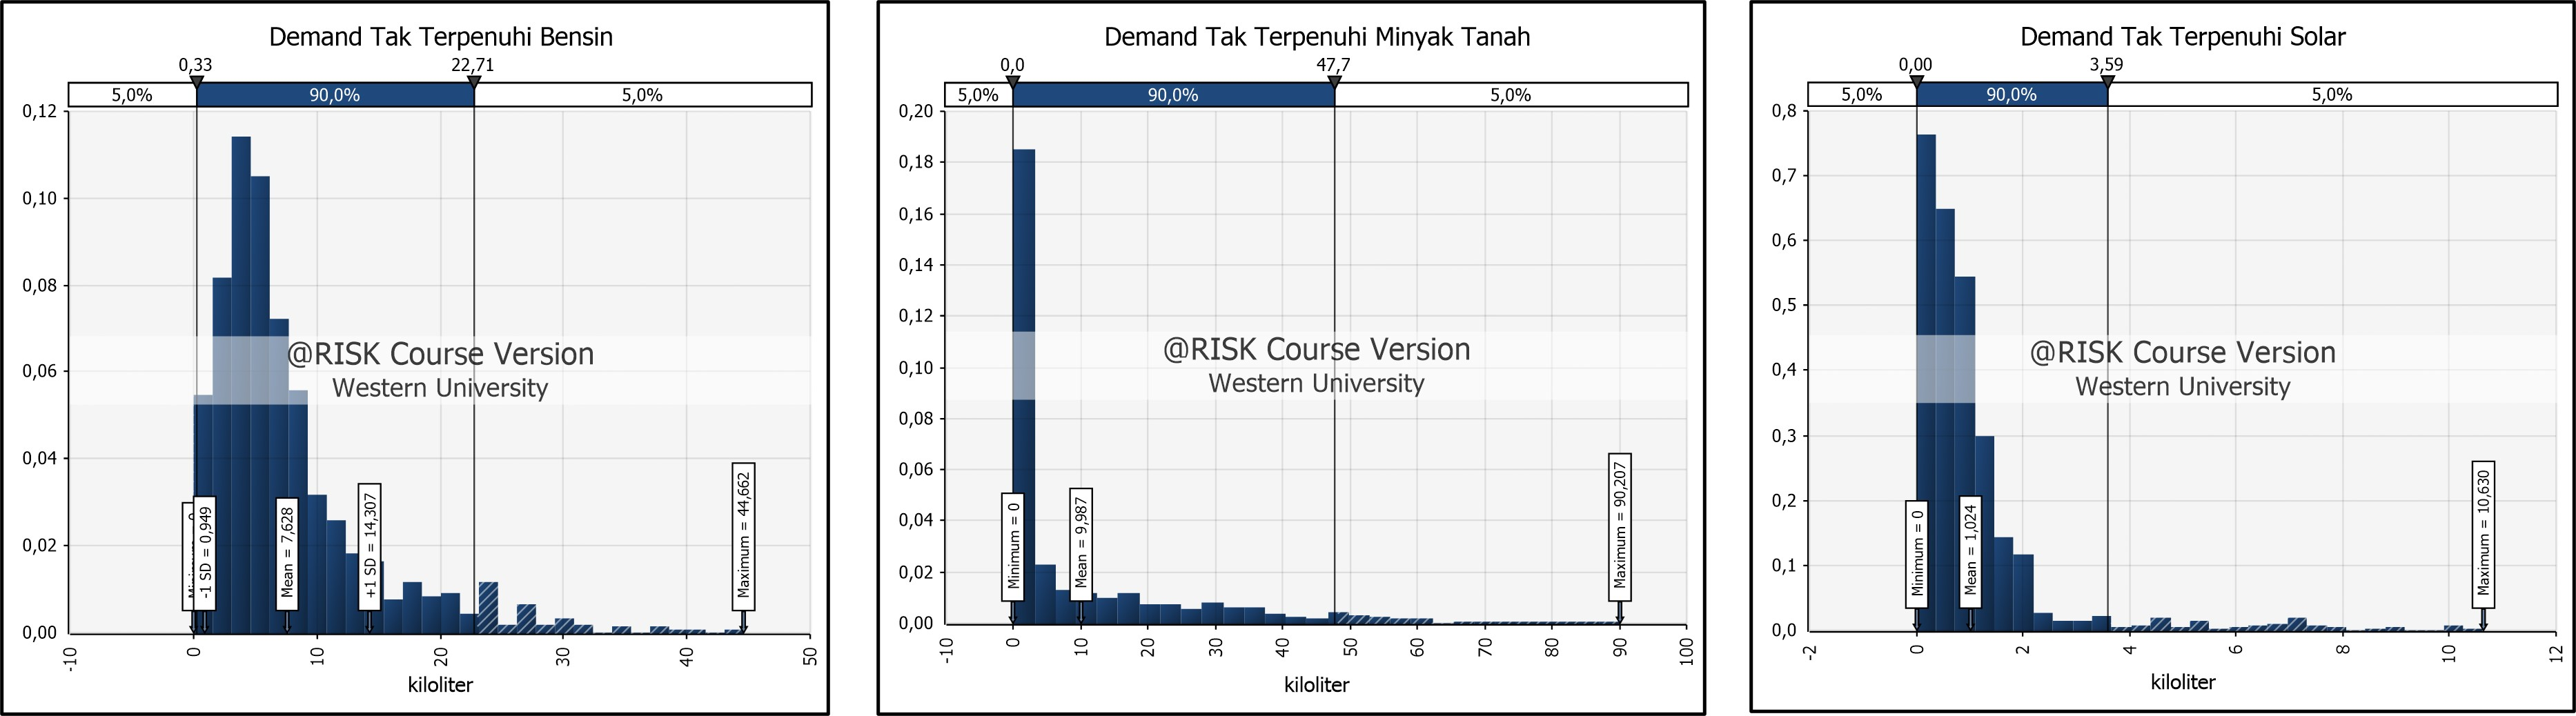
\includegraphics[width=\textwidth]{grafik/minus-bbm-baru-tangki.jpg}
        \caption{Dengan Tangki}    
    \end{subfigure}
    \caption{Hasil Simulasi Kelangkaan BBM Sistem Baru}
    \label{fig:minus-bbm-baru}
\end{figure}

Reduksi permintaan BBM yang tidak terpenuhi secara signifikan terlihat pada sistem baru dibandingkan dengan kondisi saat ini. Secara sederhana hal ini dapat dijelaskan bahwa semakin sedikit perjalanan yang dibutuhkan semakin kecil kemungkinan untuk bertemu dengan cuaca yang buruk. Namun perlu ditetapkan \emph{safety stock} yang tepat sehingga tidak terjadi kelangkaan ketika menunggu kapal datang untuk memasok.

\subsection{Perhitungan Kebutuhan Tangki Tambahan}
\label{subsec:hitungan-tangki}

Konsekuensi dari sistem yang diusulkan yakni mengurangi frekuensi kunjungan kapal adalah adanya persediaan BBM yang cukup antar kedatangan kapal. Formulasi yang digunakan untuk menghitung kebutuhan tangki adalah penyimpanan tersedia saat ini dikurangi perkalian dari jeda hari antar pemasokan dengan konsumsi harian kemudian dibulatkan keatas menyesuaikan ukuran tangki yang tersedia. Rekapitulasi kebutuhan tangki tambahan dapat dilihat pada tabel \ref{rekapitulasi-tambahan-tangki}.

\begin{table}[!htbp]
    \centering
    \caption{Rekapitulasi Tambahan Tangki yang Dibutuhkan}
    \begin{tabular}{|l|c|c|c|}
    \hline
        \textbf{Lokasi} & \textbf{Minyak Tanah [kL]} & \textbf{Solar [kL]} & \textbf{Bensin [kL]} \\ \hline
        Lakor & 50 & 0 & 0 \\ \hline
        Letti & 50 & 0 & 0 \\ \hline
        Romang & 50 & 0 & 0 \\ \hline
        Tiakur & 170 & 50 & 0 \\ \hline
        Tepa & 70 & 10 & 0 \\ \hline
    \end{tabular}
    \label{rekapitulasi-tambahan-tangki}
\end{table}

Penentuan kapasitas tangki termasuk dalam salah satu variabel peubah optimasi yang dilakukan. Hal ini diharapkan mampu memberikan ukuran tangki yang tepat jika dilihat \emph{trade off} yang muncul antara biaya kapital tangki dan biaya perjalanan kapal dalam setiap tahunnya.

\subsection{Analisis \emph{Load Factor Kapal}}
\label{subsec:load-factor-kapal}

Faktor lain yang diberikan konsideran dalam perancangan sistem pemasokan menggunakan kapal adalah \emph{load factor} dari kapal yang akan dirancang. Hal ini penting karena menggambarkan seberapa besar utilitas daya angkut kapal tersebut digunakan. Biasanya nilai \emph{load factor} yang rendah menunjukkan ukuran kapal yang dirancang masih kurang optimal.

\begin{figure}[!ht]
    \centering
    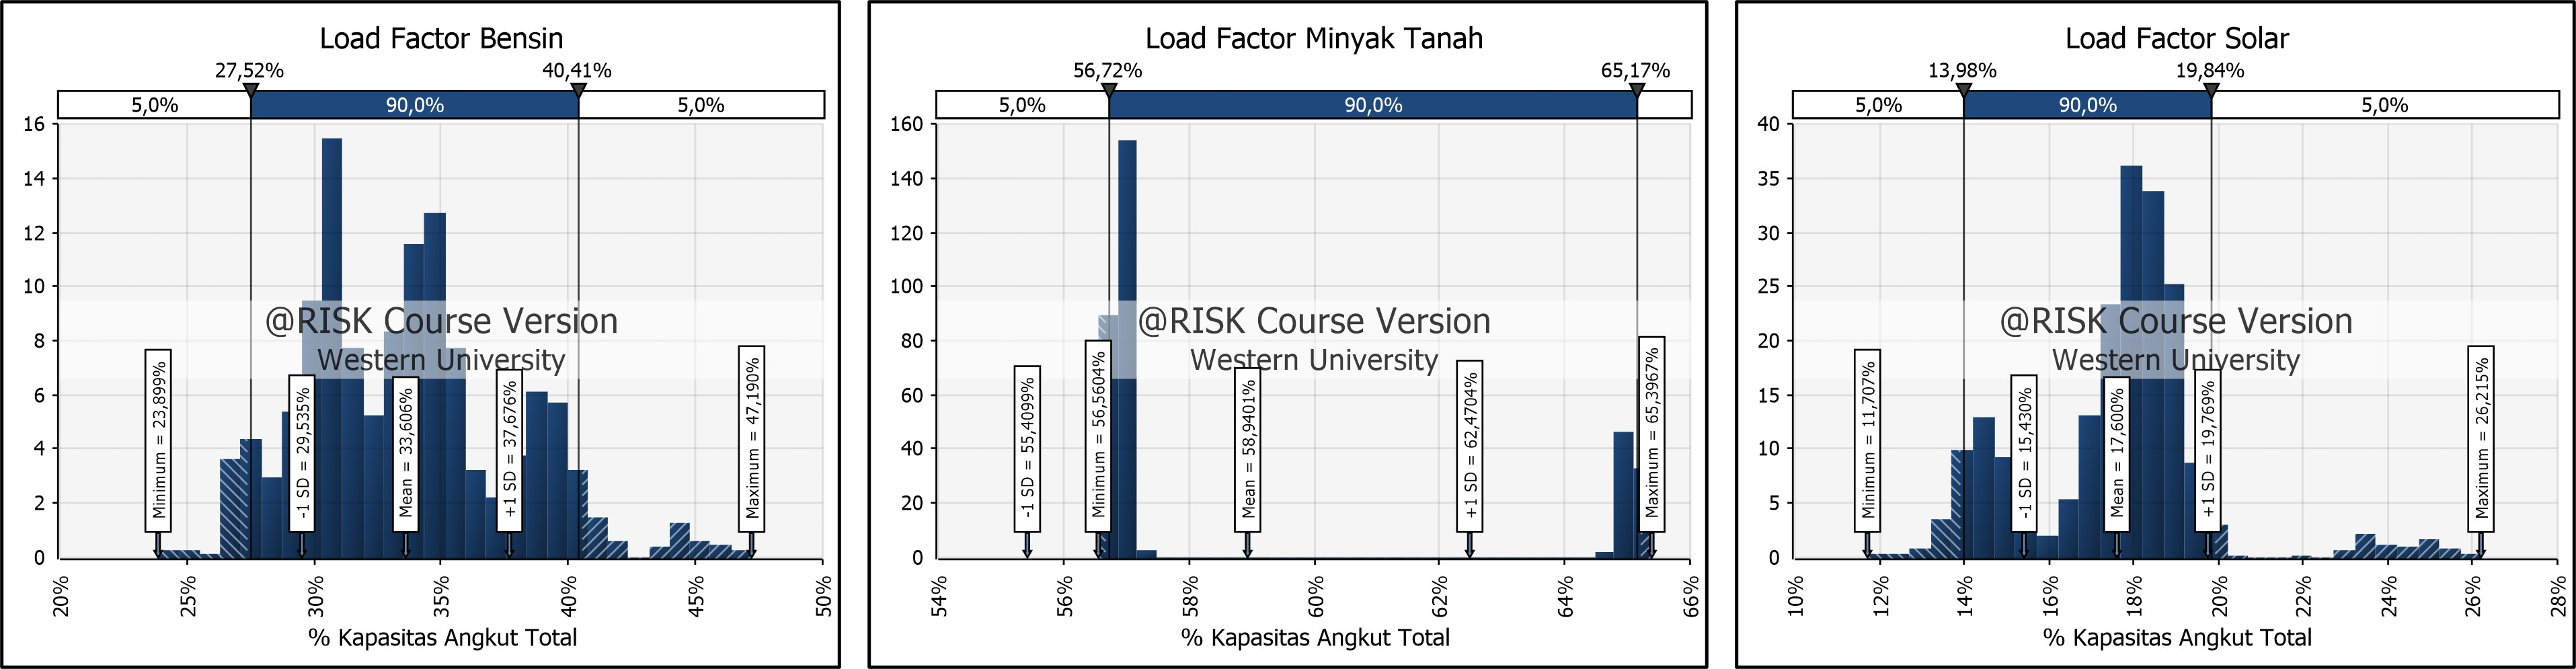
\includegraphics[width=0.95\textwidth]{grafik/load-factor-baru-tangki.jpg}
    \caption{Hasil Simulasi \emph{Load Factor} Sistem Baru}
    \label{fig:load-factor-new-tangki}
\end{figure}

Elemen \emph{load factor} ini diterjemahkan ke dalam model optimasi dengan cara mengubah kapasitas kapal yang masih kosong sebagai \emph{opportunity cost}. Biaya tersebut didapatkan dengan menghitung biaya transportasi untuk setiap liter BBM kemudian mengalikannya dengan kapasitas tangki kosong dalam setiap tahunnya. Rata-rata \emph{opportunity cost} per tahunnya sebesar 930,39 juta dengan standar deviasi 63,02 juta.
